\section{Analyzing InstructGPT/GPT-3's Emergent Arithmetic Abilities}

\begin{figure}
    \centering
    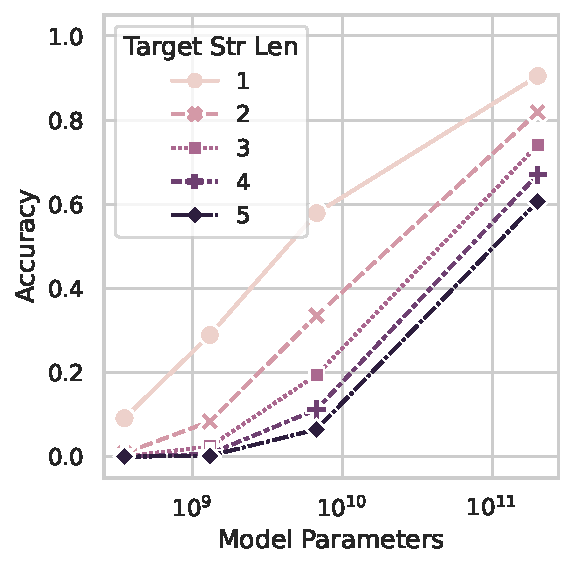
\includegraphics[width=0.26\textwidth]{figures/toy_emergence/acc_many_vs_model_size_by_target_str_len.pdf}%
    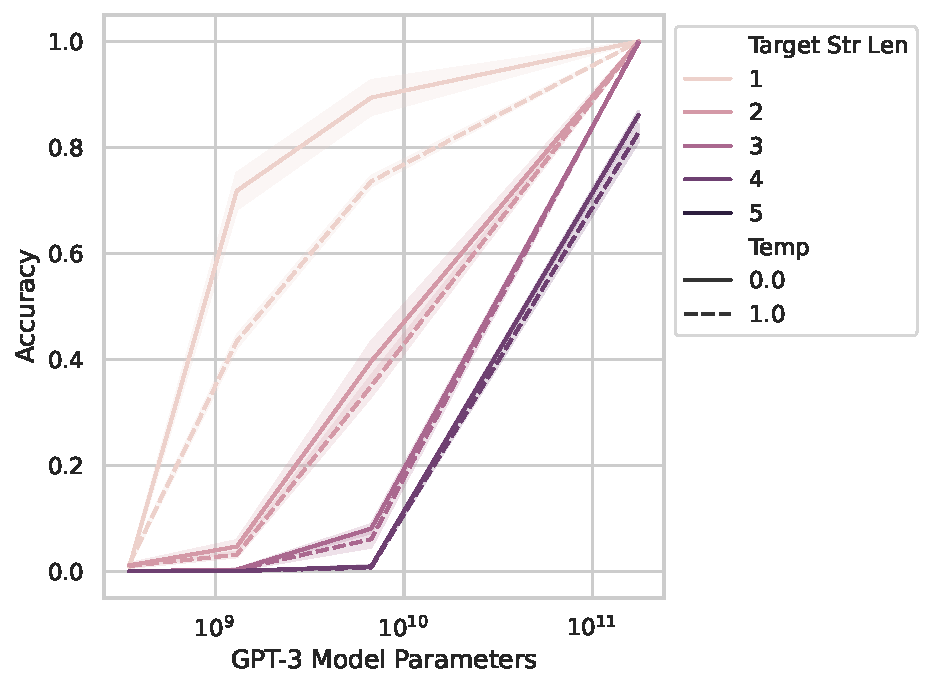
\includegraphics[width=0.35\textwidth]{figures/gpt3_integer_multiplication/multiplication_acc_vs_model_size_by_temp_by_target_str_len.pdf}%
    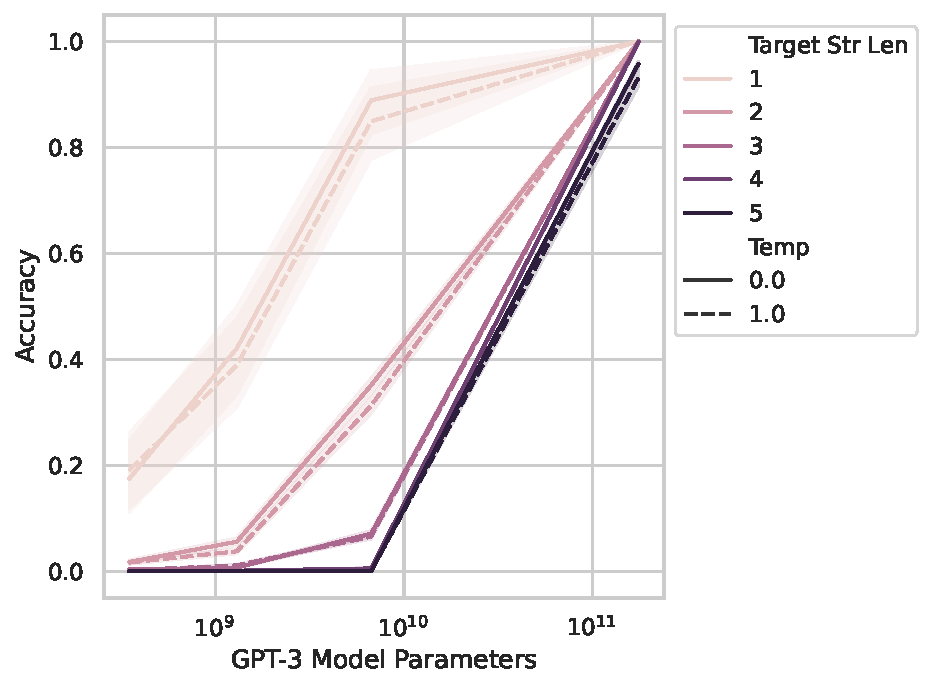
\includegraphics[width=0.35\textwidth]{figures/gpt3_integer_addition/addition_acc_vs_model_size_by_temp_by_target_str_len.pdf}
    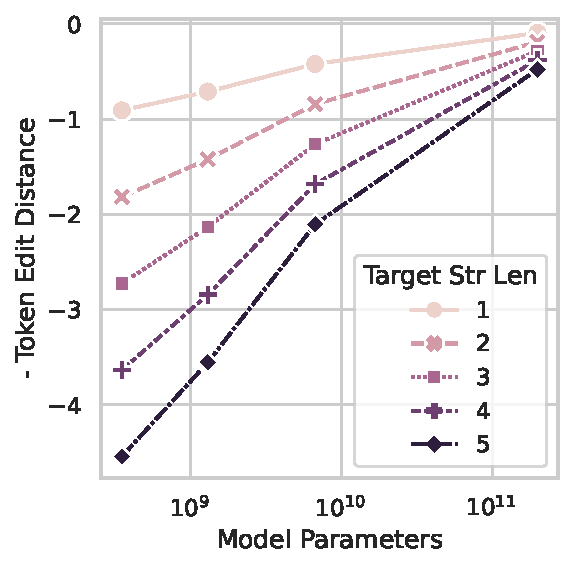
\includegraphics[width=0.26\textwidth]{figures/toy_emergence/neg_token_edit_dist_many_vs_model_size_by_target_str_len.pdf}%
    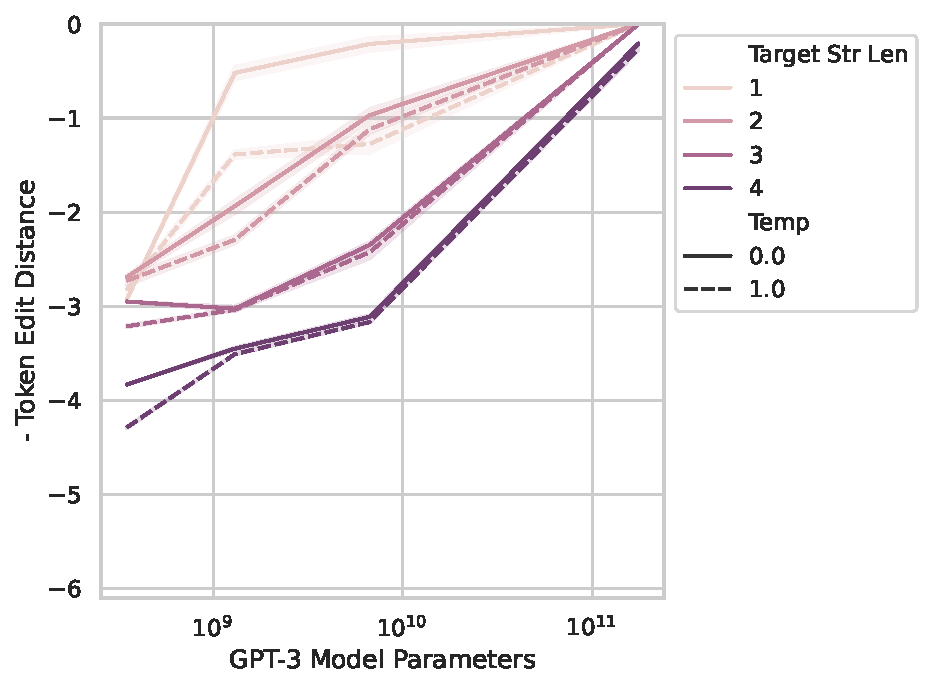
\includegraphics[width=0.35\textwidth]{figures/gpt3_integer_multiplication/multiplication_neg_token_edit_dist_vs_model_size_by_temp_by_target_str_len.pdf}%
    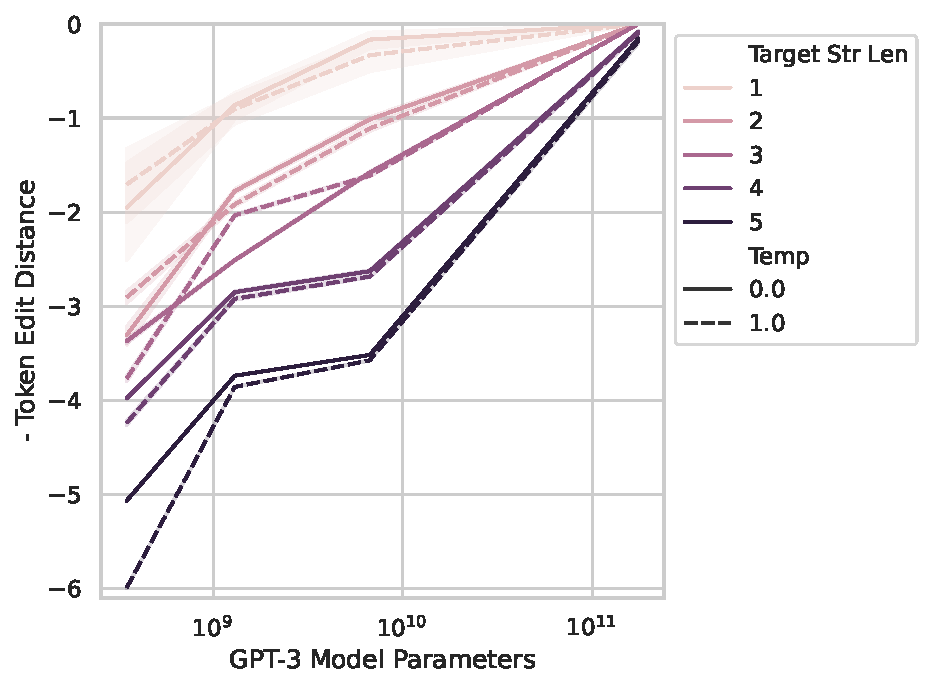
\includegraphics[width=0.35\textwidth]{figures/gpt3_integer_addition/addition_neg_token_edit_dist_vs_model_size_by_temp_by_target_str_len.pdf}
    \caption{\textbf{Claimed emergent abilities evaporate upon changing the metric.} Left to Right: Mathematical Model, 2-Integer 2-Digit Multiplication Task, 2-Integer 4-Digit Addition Task. Top: When performance is measured by a nonlinear metric (e.g., Accuracy), the InstructGPT/GPT-3 \cite{brown2020language, lowe2022instruct} family's performance appears sharp and unpredictable on longer target lengths. Bottom: When performance is instead measured by a linear metric (e.g., Token Edit Distance), the family exhibits smooth, predictable performance improvements.
    %for two claimed emergent abilities.
    }
    \label{fig:gpt_metric_change}
\end{figure}

Previous papers prominently claimed the GPT \cite{brown2020language,lowe2022instruct} family\footnote{As of 2023-03-15, 4 models with 350M, 1.3B,  6.7B, 175B parameters are available via the OpenAI API.} displays emergent abilities at integer arithmetic tasks \cite{ganguli2022predictability, srivastava2022beyond,wei2022emergent} (Fig. \ref{fig:toy_model}E).
We chose these tasks as they were prominently presented \cite{brown2020language,ganguli2022predictability,srivastava2022beyond,wei2022emergent}, and we focused on the GPT family due to it being publicly queryable.
As explained mathematically and visually in Sec. \ref{sec:alt_explanation}, our alternative explanation makes three predictions:
%
\begin{enumerate}
    \item Changing the metric from a nonlinear or discontinuous metric (Fig. \ref{fig:toy_model}CD) to a linear or continuous metric (Fig. \ref{fig:toy_model} EF) should reveal smooth, continuous, predictable performance improvement with model scale.
    \item For nonlinear metrics, increasing the resolution of measured model performance by increasing the test dataset size should reveal smooth, continuous, predictable model improvements \textit{commensurate with the predictable nonlinear effect of the chosen metric}.
    \item Regardless of metric, increasing the target string length should predictably affect the model's performance as a function of the length-1 target performance: approximately geometrically for accuracy and approximately quasilinearly for token edit distance.
\end{enumerate}

To test these predictions, we collected outputs from the InstructGPT/GPT-3 family on two tasks: 2-shot multiplication between two 2-digit integers and 2-shot addition between two 4-digit integers.
% We chose 2-shot prompting arbitrarily and were unable to experiment more broadly due to financial constraints.

\begin{figure}
    \centering
    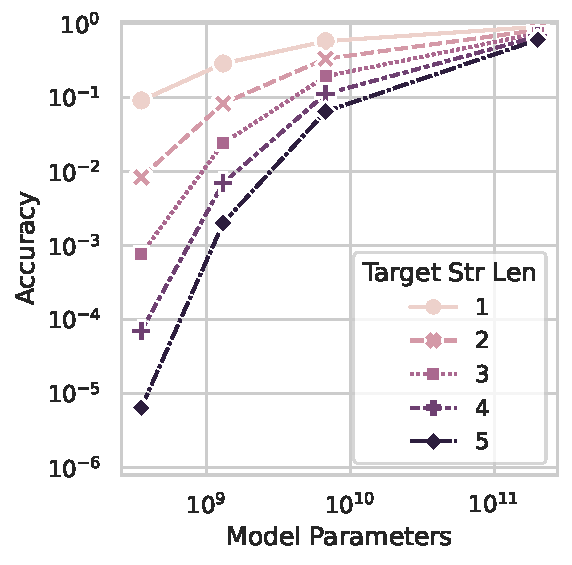
\includegraphics[width=0.26\textwidth]{figures/toy_emergence/acc_log_many_vs_model_size_by_target_str_len.pdf}%
    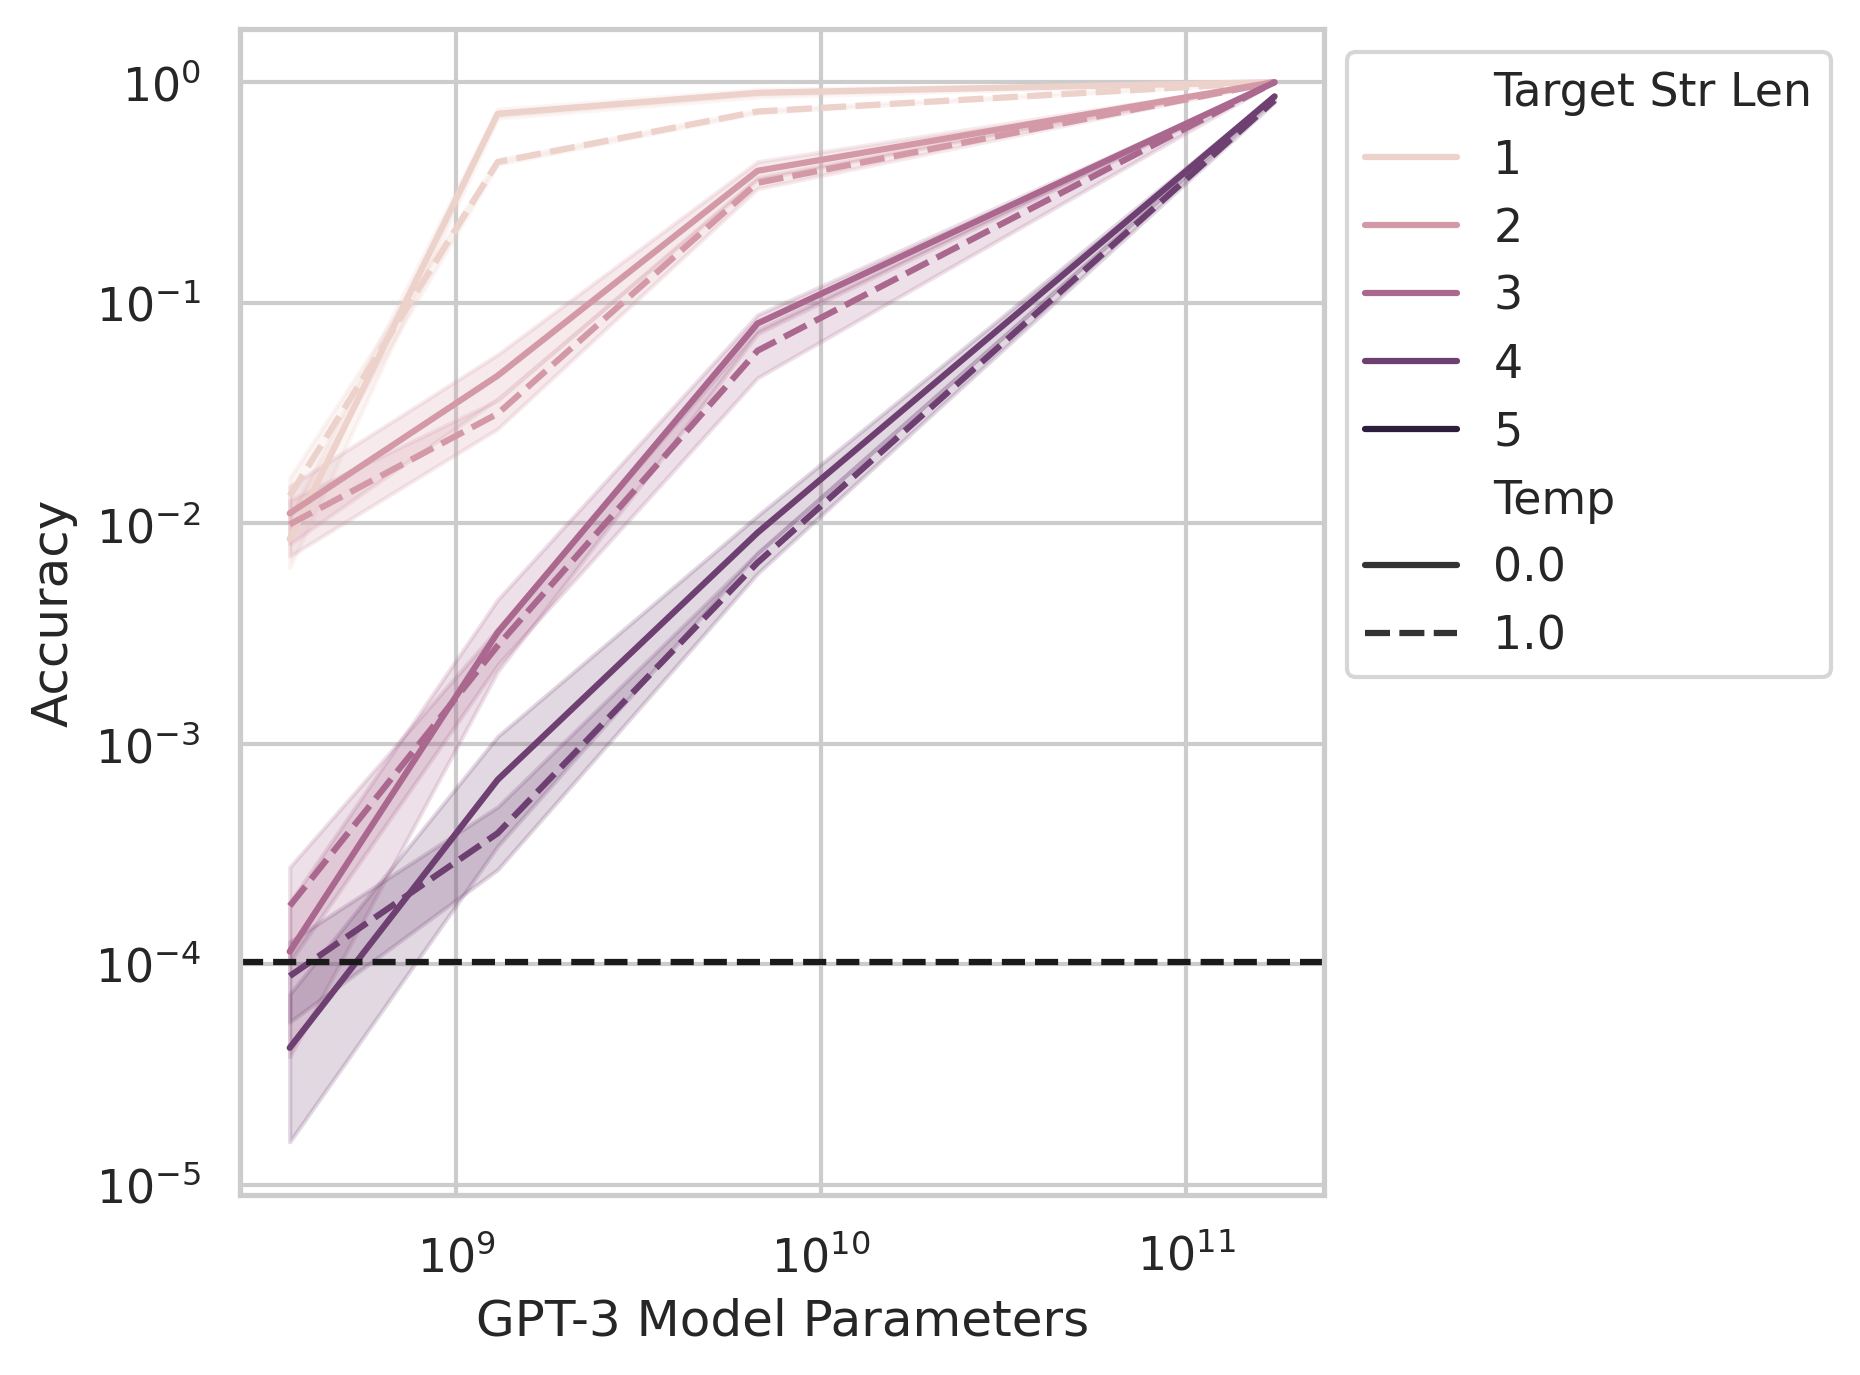
\includegraphics[width=0.35\textwidth]{figures/gpt3_integer_multiplication/multiplication_acc_log_vs_model_size_by_temp_by_target_str_len.png}%
    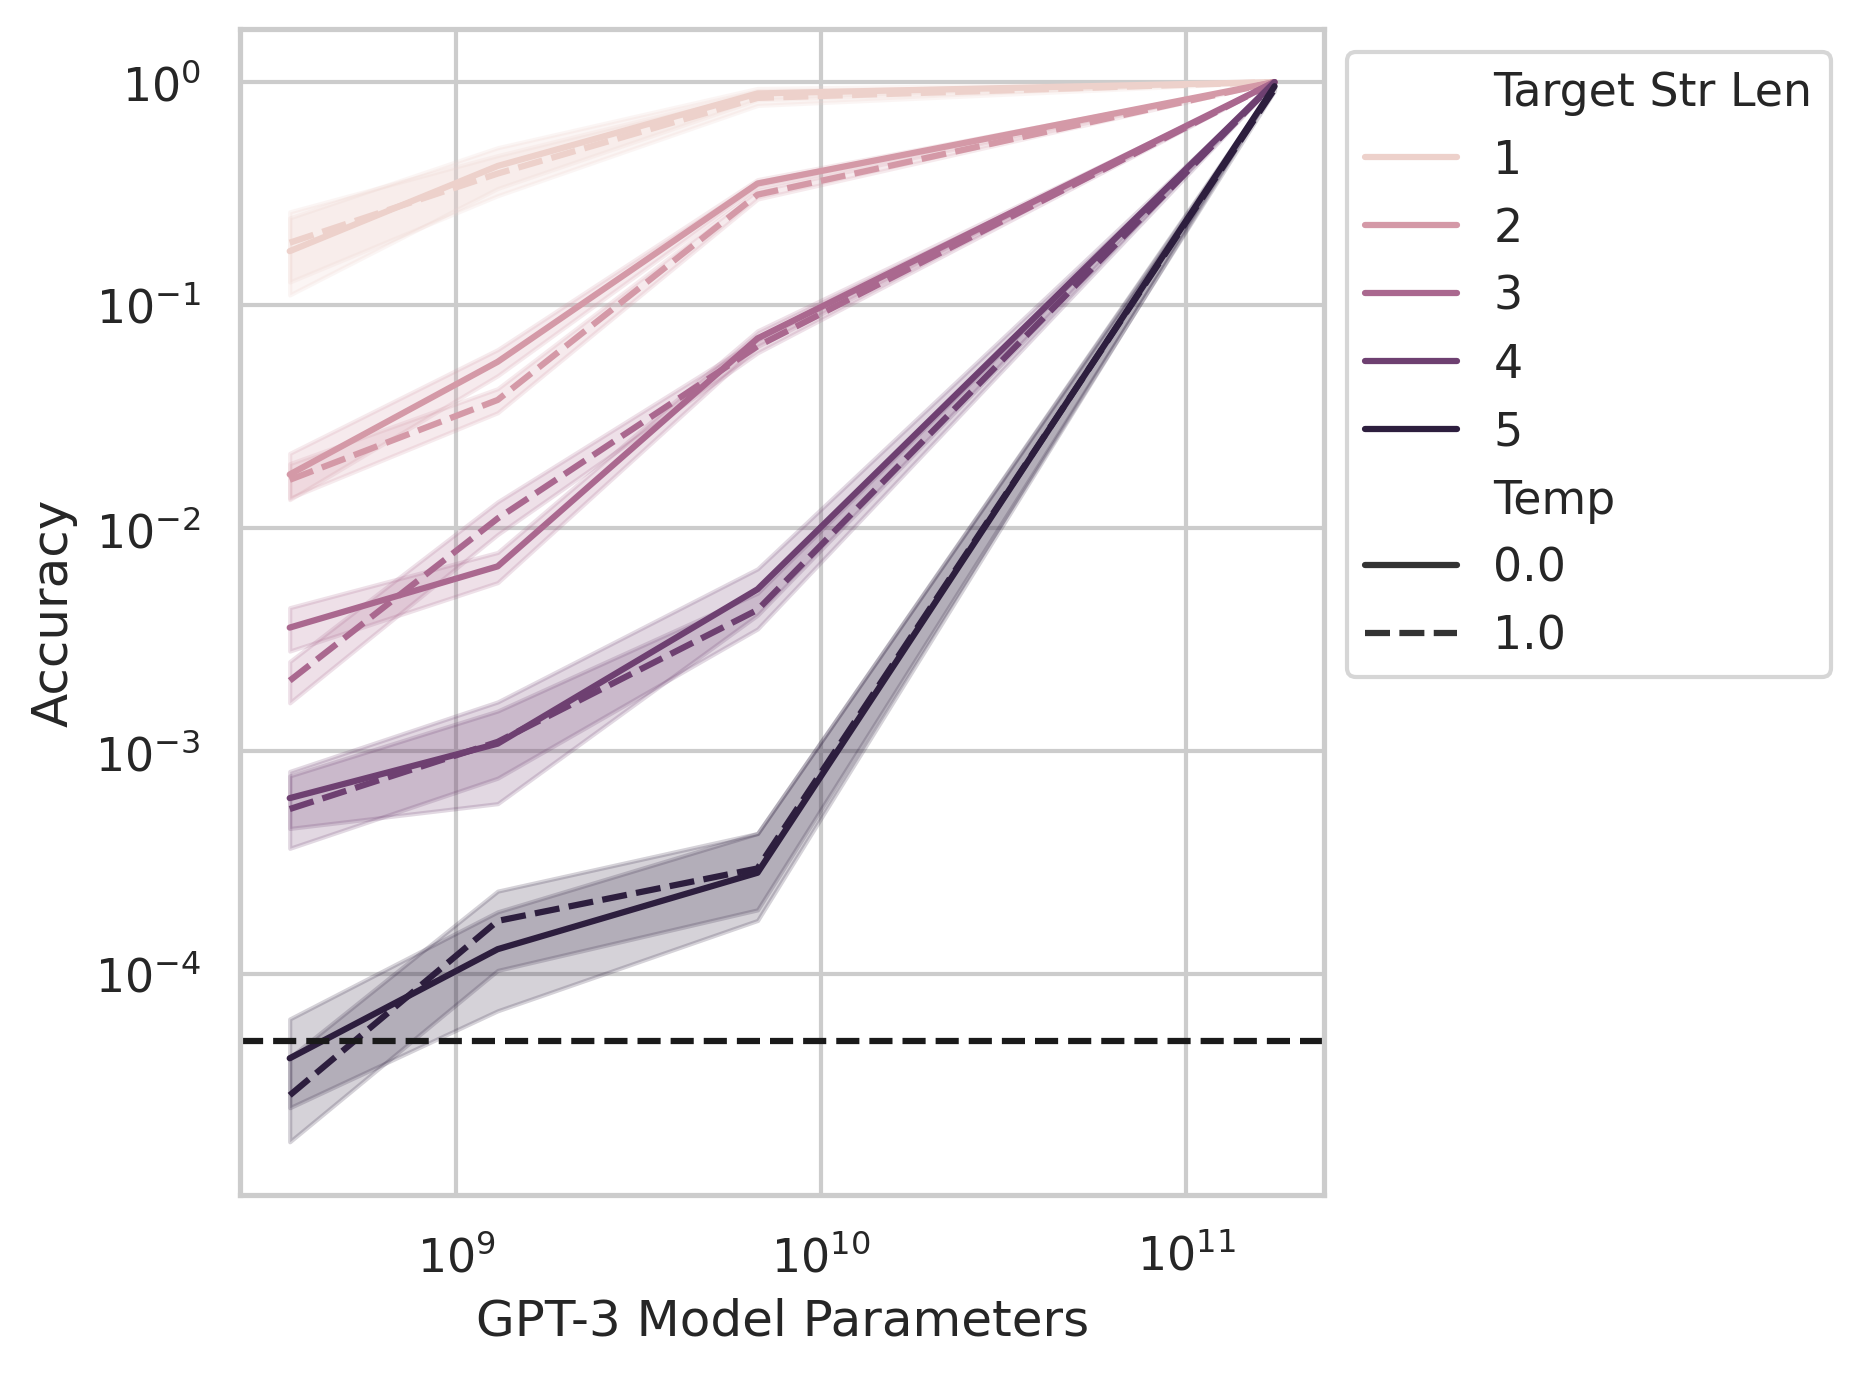
\includegraphics[width=0.35\textwidth]{figures/gpt3_integer_addition/addition_acc_log_vs_model_size_by_temp_by_target_str_len.png}
    \caption{\textbf{Claimed emergent abilities evaporate upon using better statistics.} Left to Right: Mathematical Model, 2-Integer 2-Digit Multiplication Task, 2-Integer 4-Digit Addition Task. Based on the predictable effect Accuracy has on performance, measuring performance requires high resolution. Generating additional test data increases the resolution and reveals that even on Accuracy, the InstructGPT/GPT-3 family's \cite{brown2020language, lowe2022instruct} performance is above chance and improves in a smooth, continuous, predictable manner that qualitatively matches the mathematical model.}
    \label{fig:gpt_improve_resolution}
\end{figure}

% \begin{figure}
%     \centering
%     \begin{center}
%         4-Digit Integer Addition \quad \quad \quad \quad \quad \quad 2-Digit Integer Multiplication
%     \end{center}
%     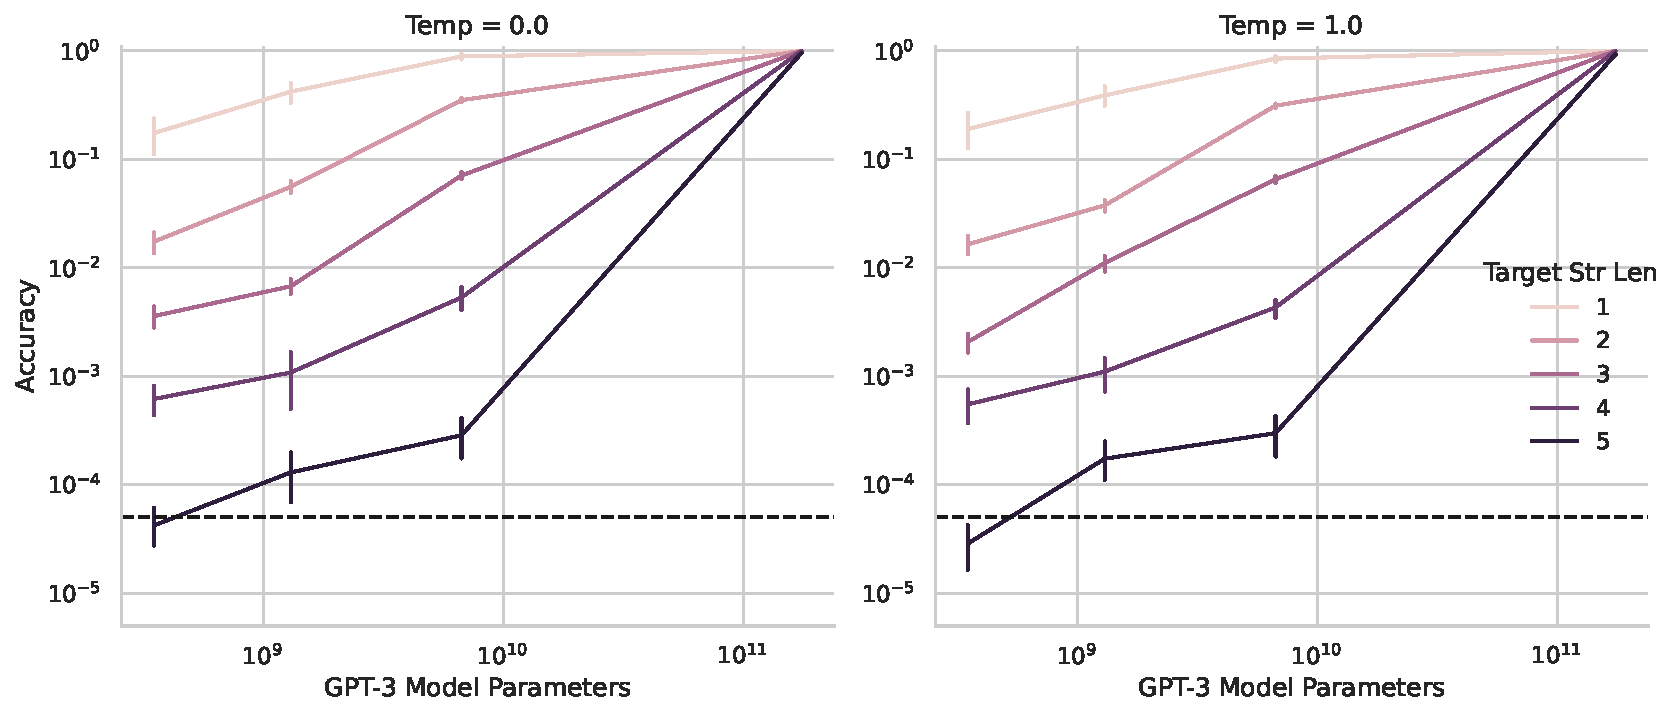
\includegraphics[width=0.49\textwidth]{figures/gpt3_integer_addition/addition_acc_vs_model_size_by_target_str_len.pdf}
%     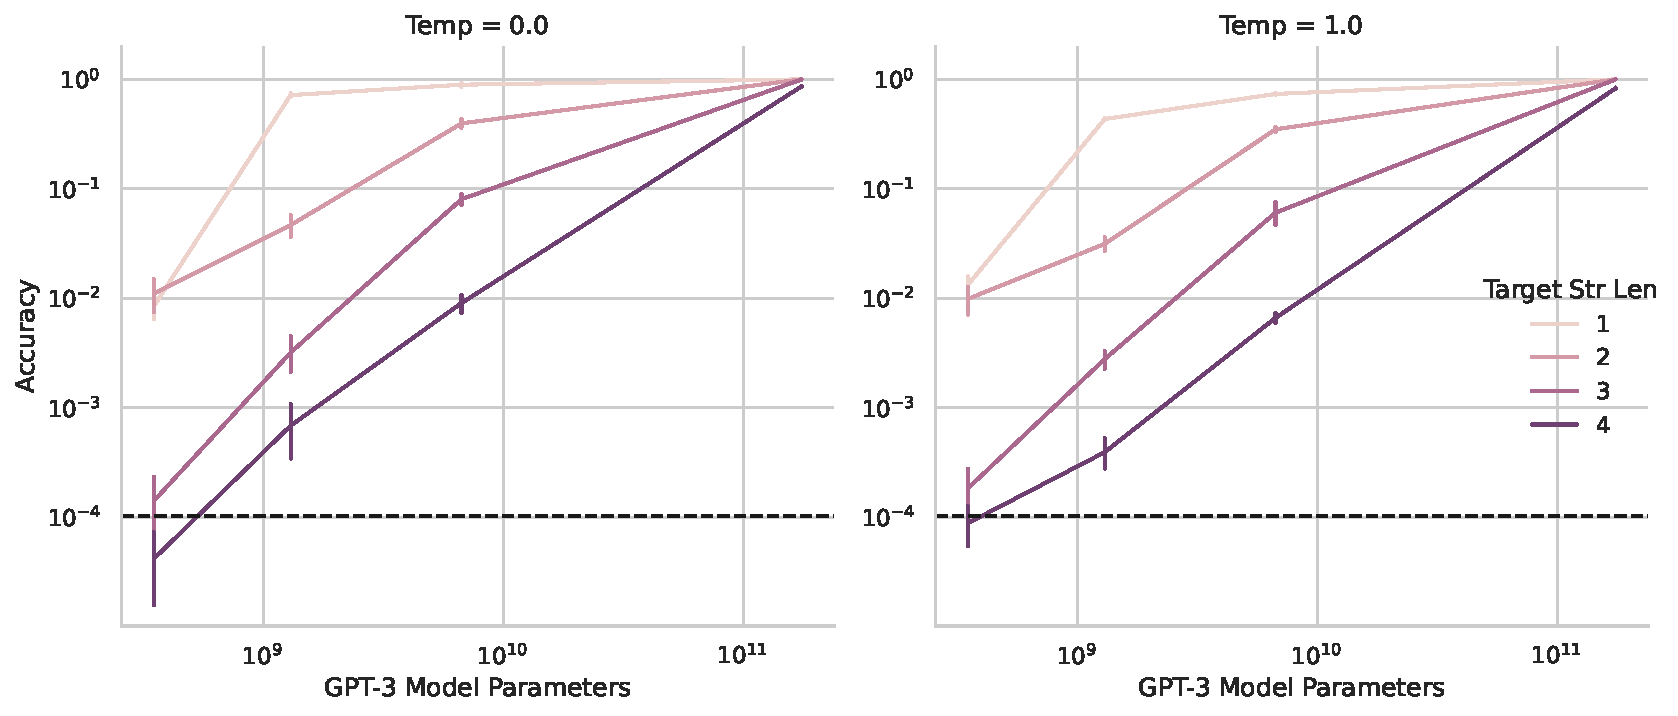
\includegraphics[width=0.49\textwidth]{figures/gpt3_integer_multiplication/multiplication_acc_vs_model_size_by_target_str_len.pdf}
%     \caption{\textbf{Better estimating accuracy with more test data reveals that performance changes are smooth, continuous and predictable}.}
%     \label{fig:gpt_improve_resolution}
% \end{figure}


\paragraph{Prediction: Emergent Abilities Disappear With Different Metrics}
On both arithmetic tasks, the GPT family displays emergent abilities if the target has 4 or 5 digits and if the metric is Accuracy (Fig. \ref{fig:gpt_metric_change}, top) \cite{brown2020language, ganguli2022predictability,wei2022emergent}. However, if one changes from nonlinear Accuracy to linear Token Edit Distance \textit{while keeping the models' outputs fixed}, the family's performance smoothly, continuously and predictably improves with increasing scale (Fig. \ref{fig:gpt_metric_change}, bottom). This confirms our first prediction and supports our alternative explanation that the source of emergent abilities is the researcher's choice of metric, \textit{not changes in the model family's outputs}. We also observe that under Token Edit Distance, increasing the length of the target string from 1 to 5 predictably decreases the family's performance in an approximately quasilinear manner, confirming the first half of our third prediction.

% \begin{figure}
%     \centering
%     \begin{minipage}{.25\textwidth}
%         \centering
%         Mathematical Model
%         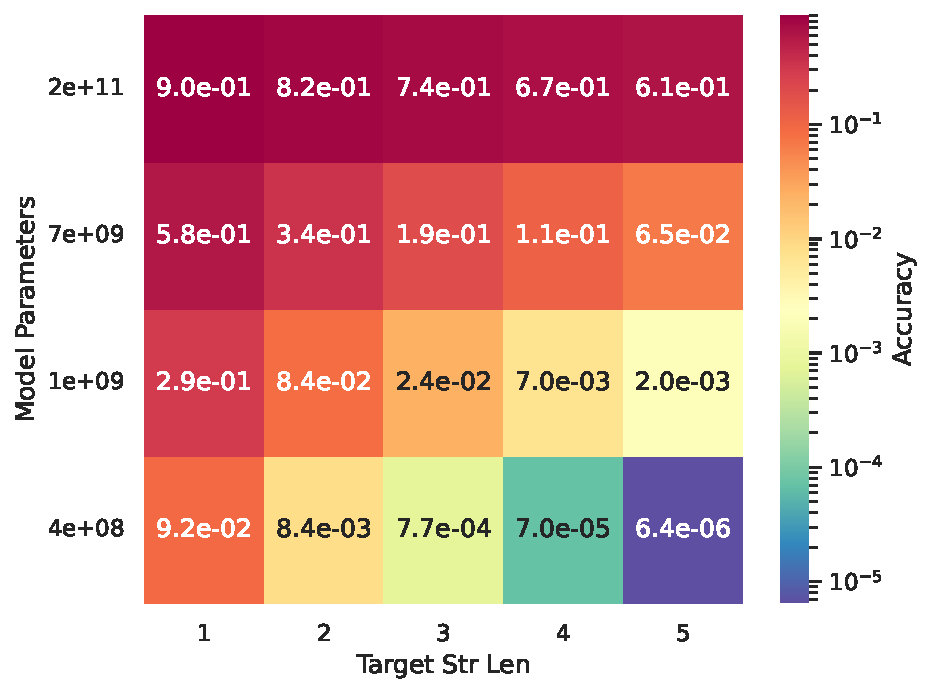
\includegraphics[width=0.95\textwidth]{figures/toy_emergence/heatmap_acc_by_model_size_by_target_str_len.pdf}
%     \end{minipage}\hfill
%     \begin{minipage}{0.36\textwidth}
%         \centering
%         4-Digit Integer Addition
%         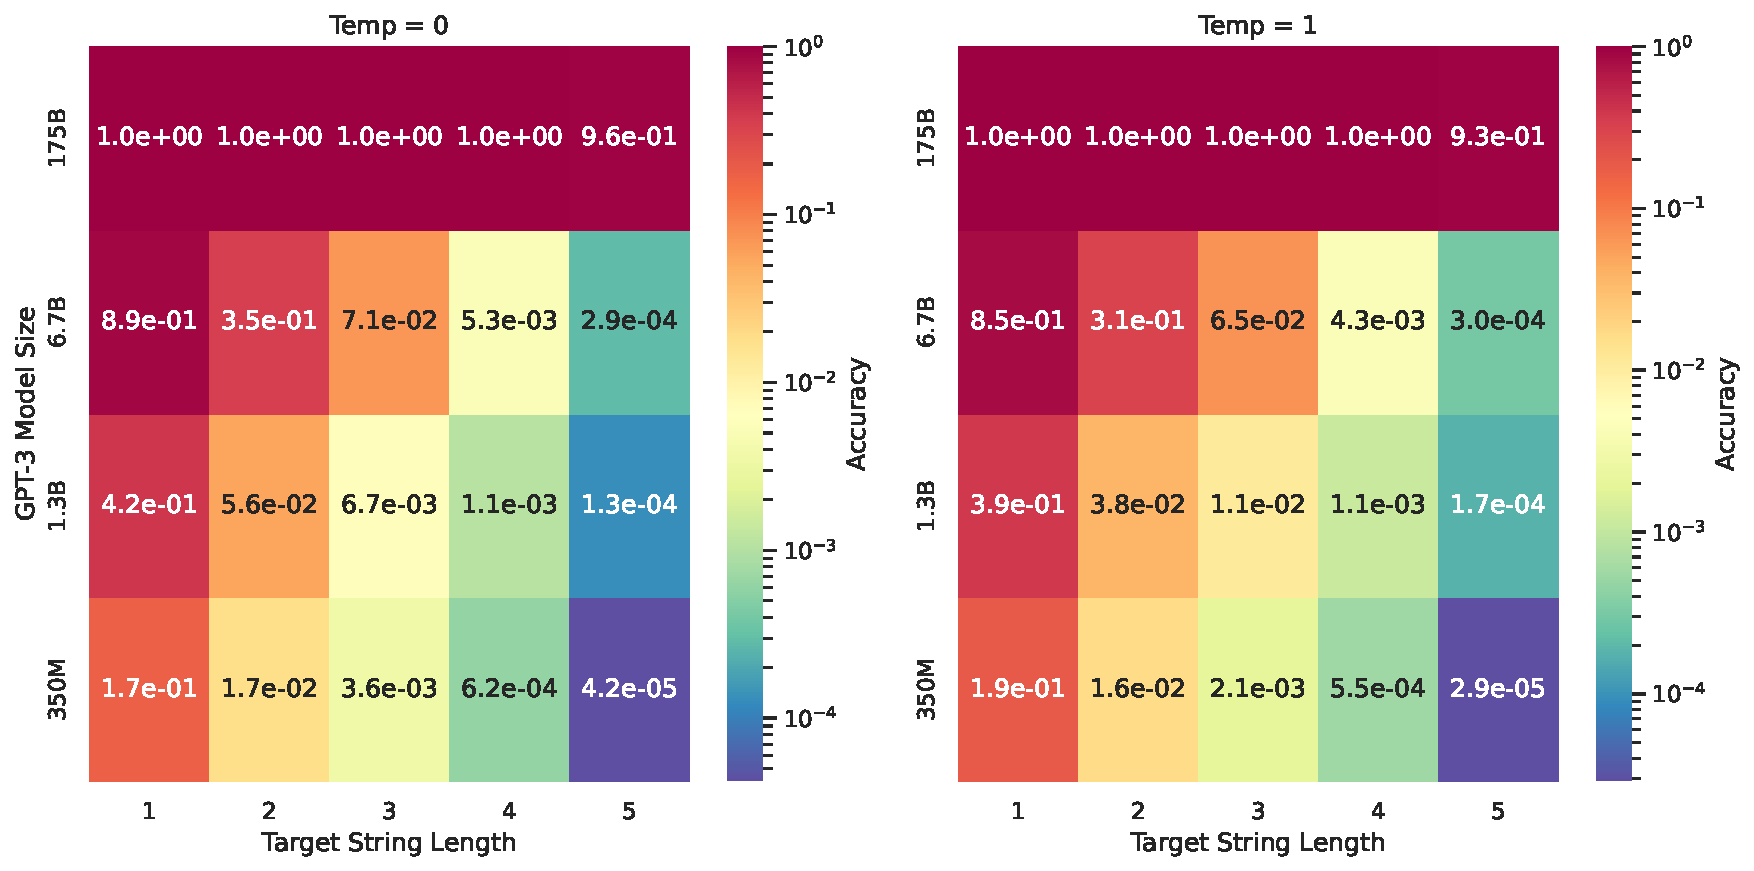
\includegraphics[width=0.95\textwidth]{figures/gpt3_integer_addition/heatmap_acc_by_model_size_by_target_str_len.pdf}
%     \end{minipage}\hfill
%     \begin{minipage}{0.36\textwidth}
%         \centering
%         2-Digit Integer Multiplication
%         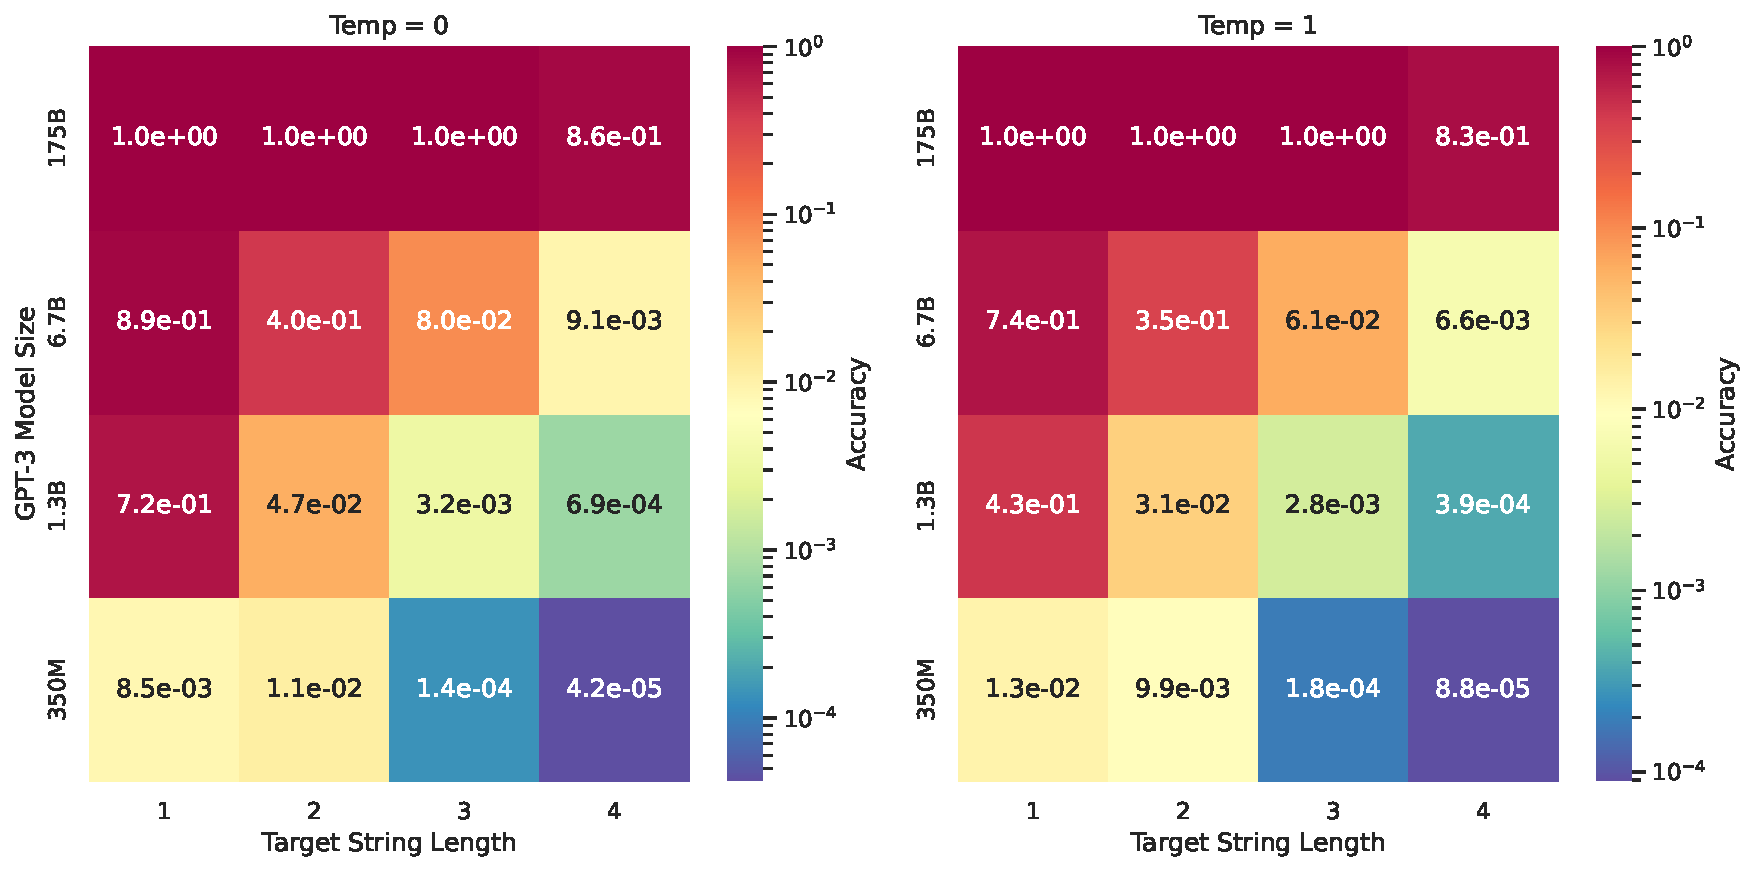
\includegraphics[width=0.95\textwidth]{figures/gpt3_integer_multiplication/heatmap_acc_by_model_size_by_target_str_len.pdf}
%     \end{minipage}
%     \caption{\textbf{}}
%     \label{fig:my_label}
% \end{figure}



\paragraph{Prediction: Emergent Abilities Disappear With Better Statistics}

We next tested our second prediction: that even on nonlinear metrics such as accuracy, smaller models do not have zero accuracy, but rather have non-zero above-chance accuracy \textit{commensurate with choosing to use accuracy as the metric}. In order to accurately measure models' accuracy, we increased the resolution by generating additional test data, and found that on both arithmetic tasks, all models in the InstructGPT/GPT-3 family achieve above-chance accuracy (Fig. \ref{fig:gpt_improve_resolution}). This confirms our second prediction. We also observe that as the target string length increases, the accuracy falls approximately geometrically with the length of the target string, confirming the second half of our third prediction. These results additionally demonstrate that the researcher's choice of metric has the effect that one should predict accuracy to have, i.e., geometric decay with the target length.

% \subsection{GPT-3's per-token probability of selecting the correct token}

% \begin{figure}
%     \centering
%     \begin{minipage}{.32\textwidth}
%         \centering
%         Mathematical Model
%         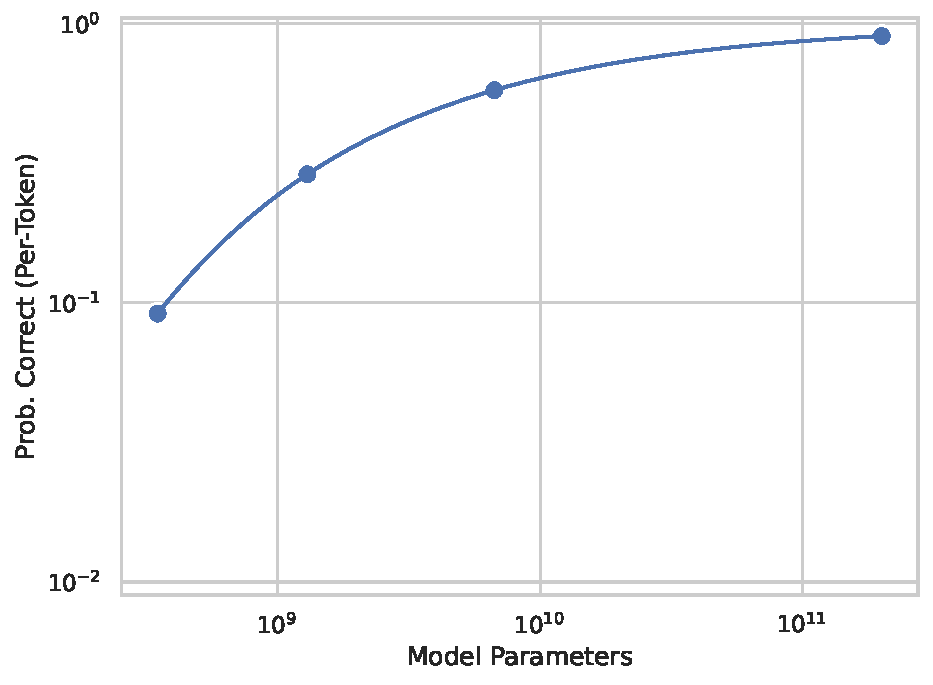
\includegraphics[width=0.95\textwidth]{figures/toy_emergence/prob_correct_per_token_vs_model_size.pdf}
%     \end{minipage}%
%     \begin{minipage}{0.32\textwidth}
%         \centering
%         4-Digit Integer Addition
%         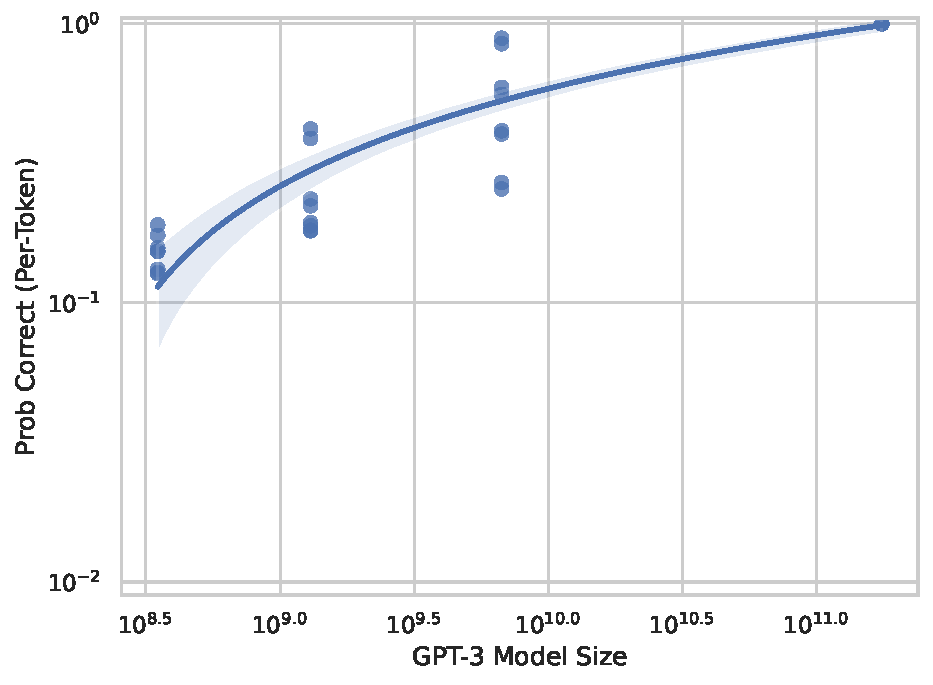
\includegraphics[width=0.95\textwidth]{figures/gpt3_integer_addition/prob_correct_per_token_vs_model_size.pdf}
%     \end{minipage}%
%     \begin{minipage}{0.35\textwidth}
%         \centering
%         2-Digit Integer Multiplication
%         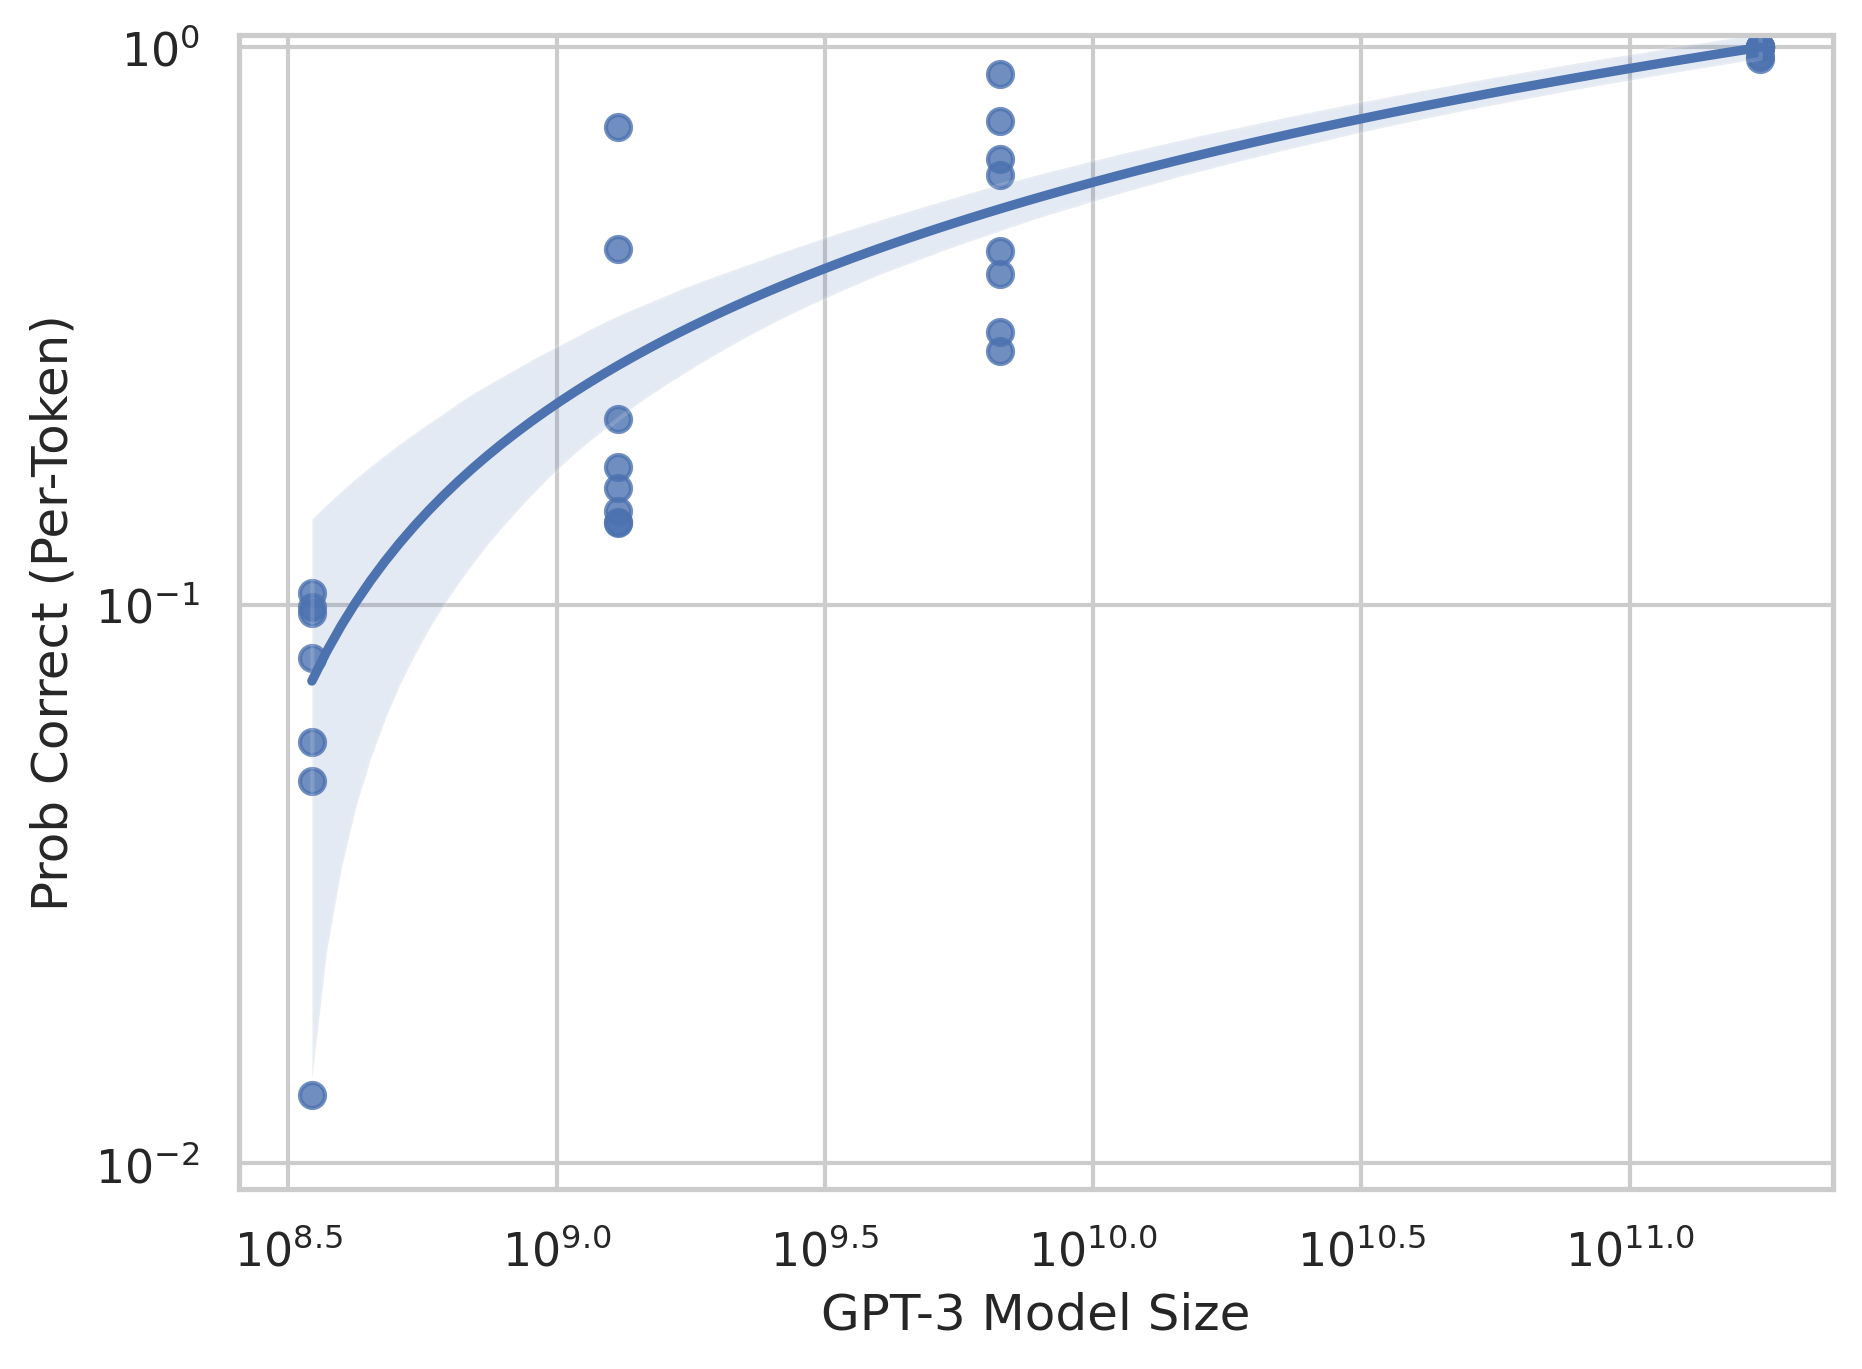
\includegraphics[width=0.95\textwidth]{figures/gpt3_integer_multiplication/prob_correct_per_token_vs_model_size.png}
%     \end{minipage}
%     \caption{Are these figures worth including? Unclear... Probably not}
%     \label{fig:my_label}
% \end{figure}

% As an additional test for our mathematical model, we can leverage the fact that the GPT-3 family follows a neural scaling law \cite{brown2020language} to compute the family's per-token probability of selecting the correct token in two different ways. In the first approach, we can invert the published test cross entropies to recover the per-token probability correct; in the second approach, we can take the model's output generated strings and compute the per-token probability correct.

